\documentclass{article}
\usepackage{graphicx}
\title{ECE 1895 - ASSIGNMENT 2 REPORT}
\author{Yinhao Qian}
\begin{document}
	\maketitle
	\section{Screenshots of your schematic:}
	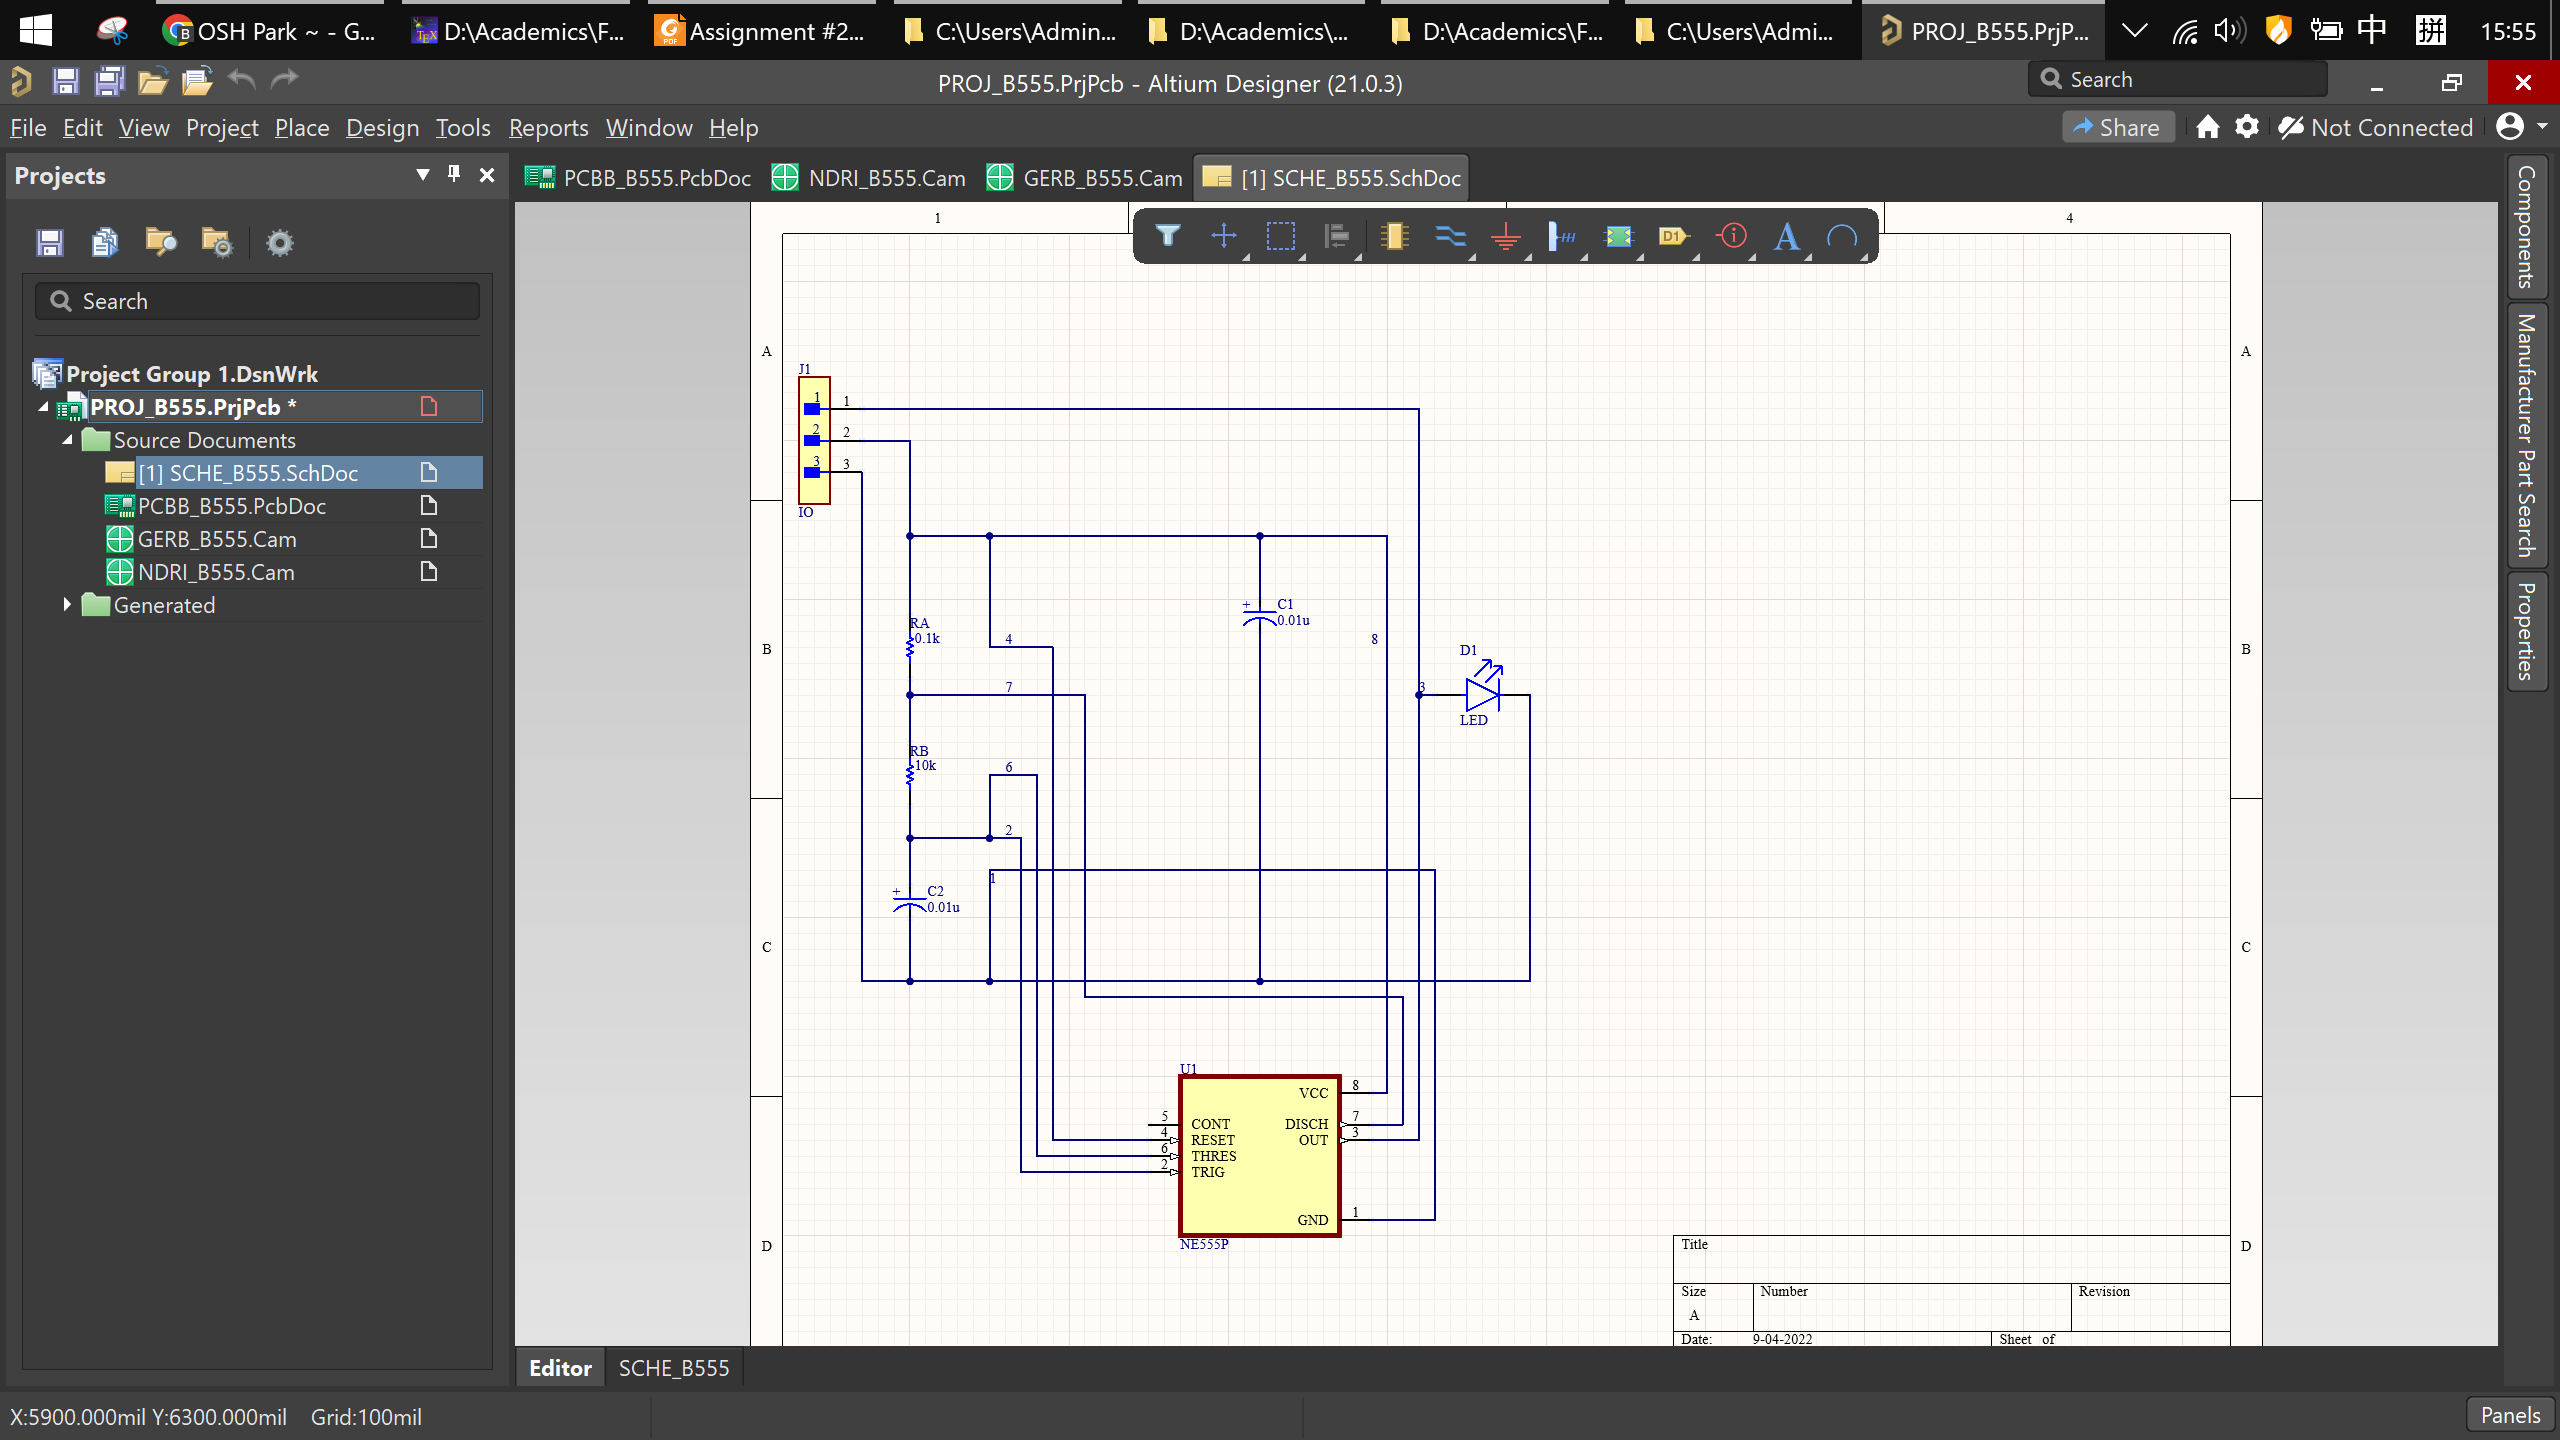
\includegraphics[width=\columnwidth]{SCHE_B555}
	I'll use a three-pin header named J1 for voltage source, output and ground. 
	Pin 1 provides the output voltage, \textbf{which provides a way for the user to access the output waveform of the 555-timer}. Pin 2 connects to the source voltage, \textbf{which provides a way for the user to supply power.} Pin 3 connects to ground, \textbf{which provides a way for the user to supply ground.}
	\section{Screenshots of your PCB:}
	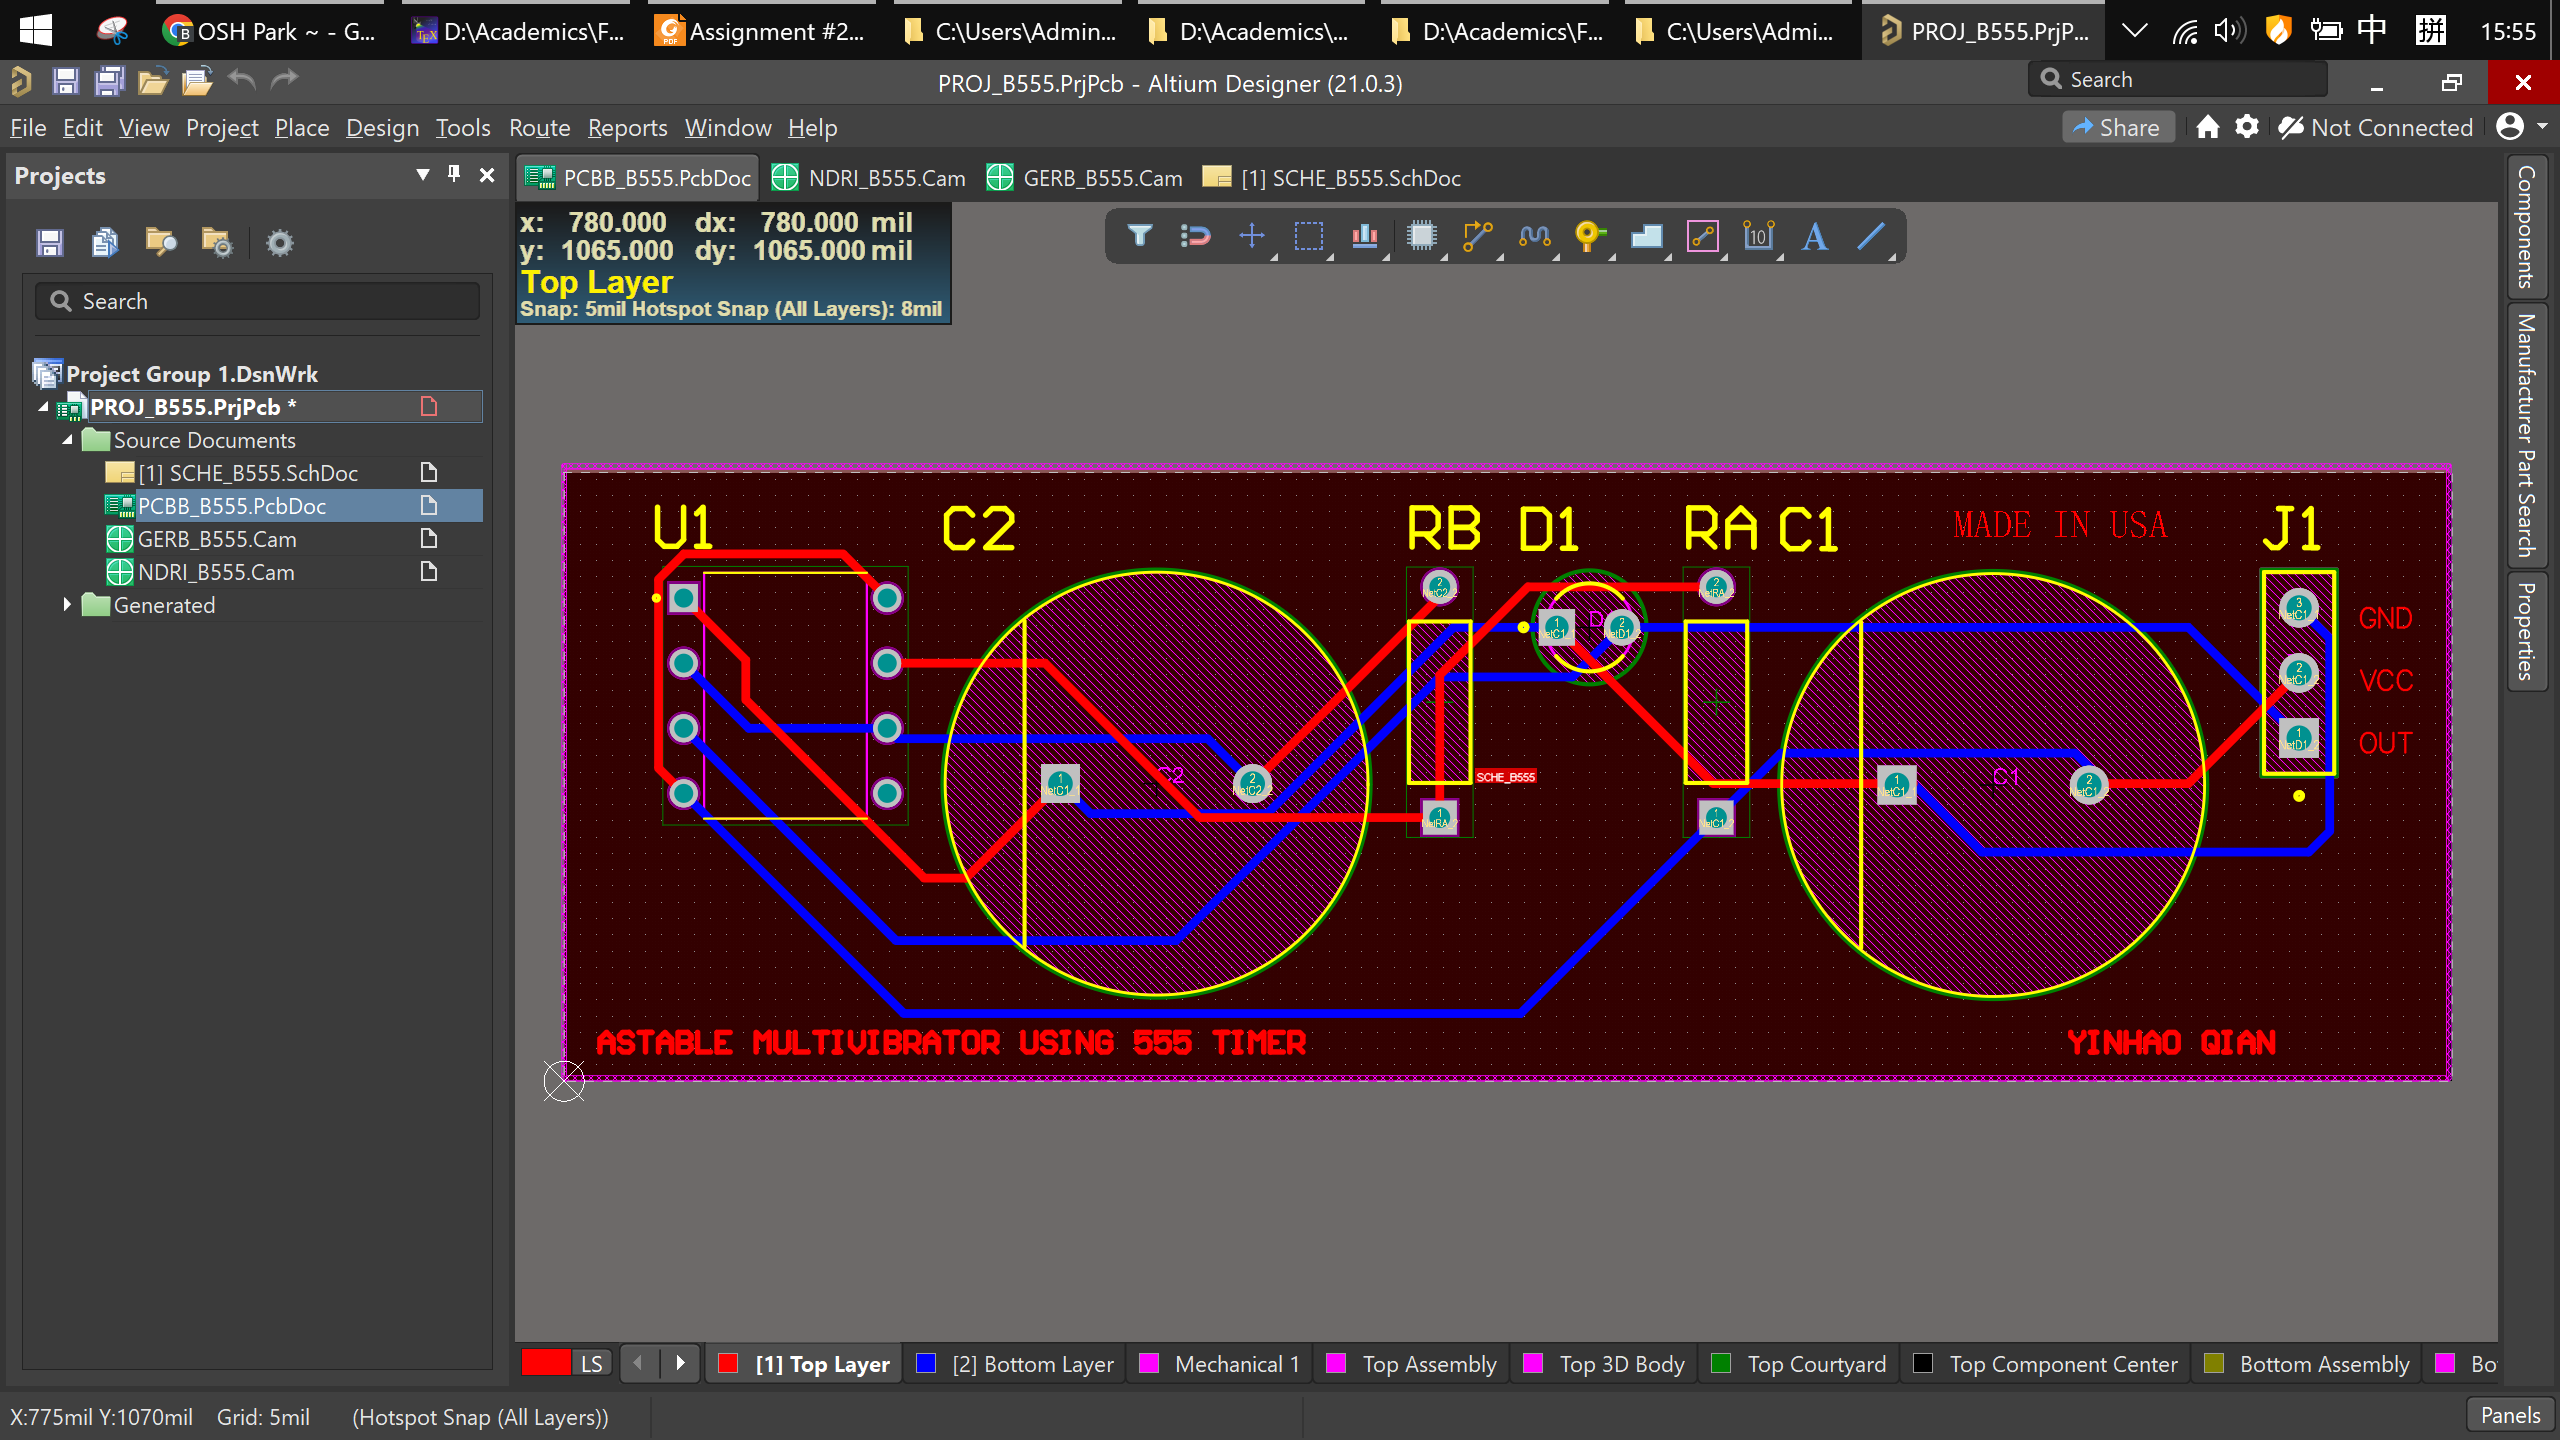
\includegraphics[width=\columnwidth]{PCBB_B555}
	Each designated components map to unique ones from schematics, so it shows the PCB design have \textbf{components that match that of your schematic}.\newline\newline
	\subsubsection{A description of your PCB}
	The layout of each components remains unchanged since changing the layout manually does not necessary improve the wiring efficiency. I have also added some annotations on the bottom of the PCB board to make it "a bit more professional". The only parts that user should concern about is the three pins on the top right corner. I have added annotations to each pin to make sure they are connected correctly by the user.
	\section{Screenshots of your report logs showing no connectivity or design rule violations:}
	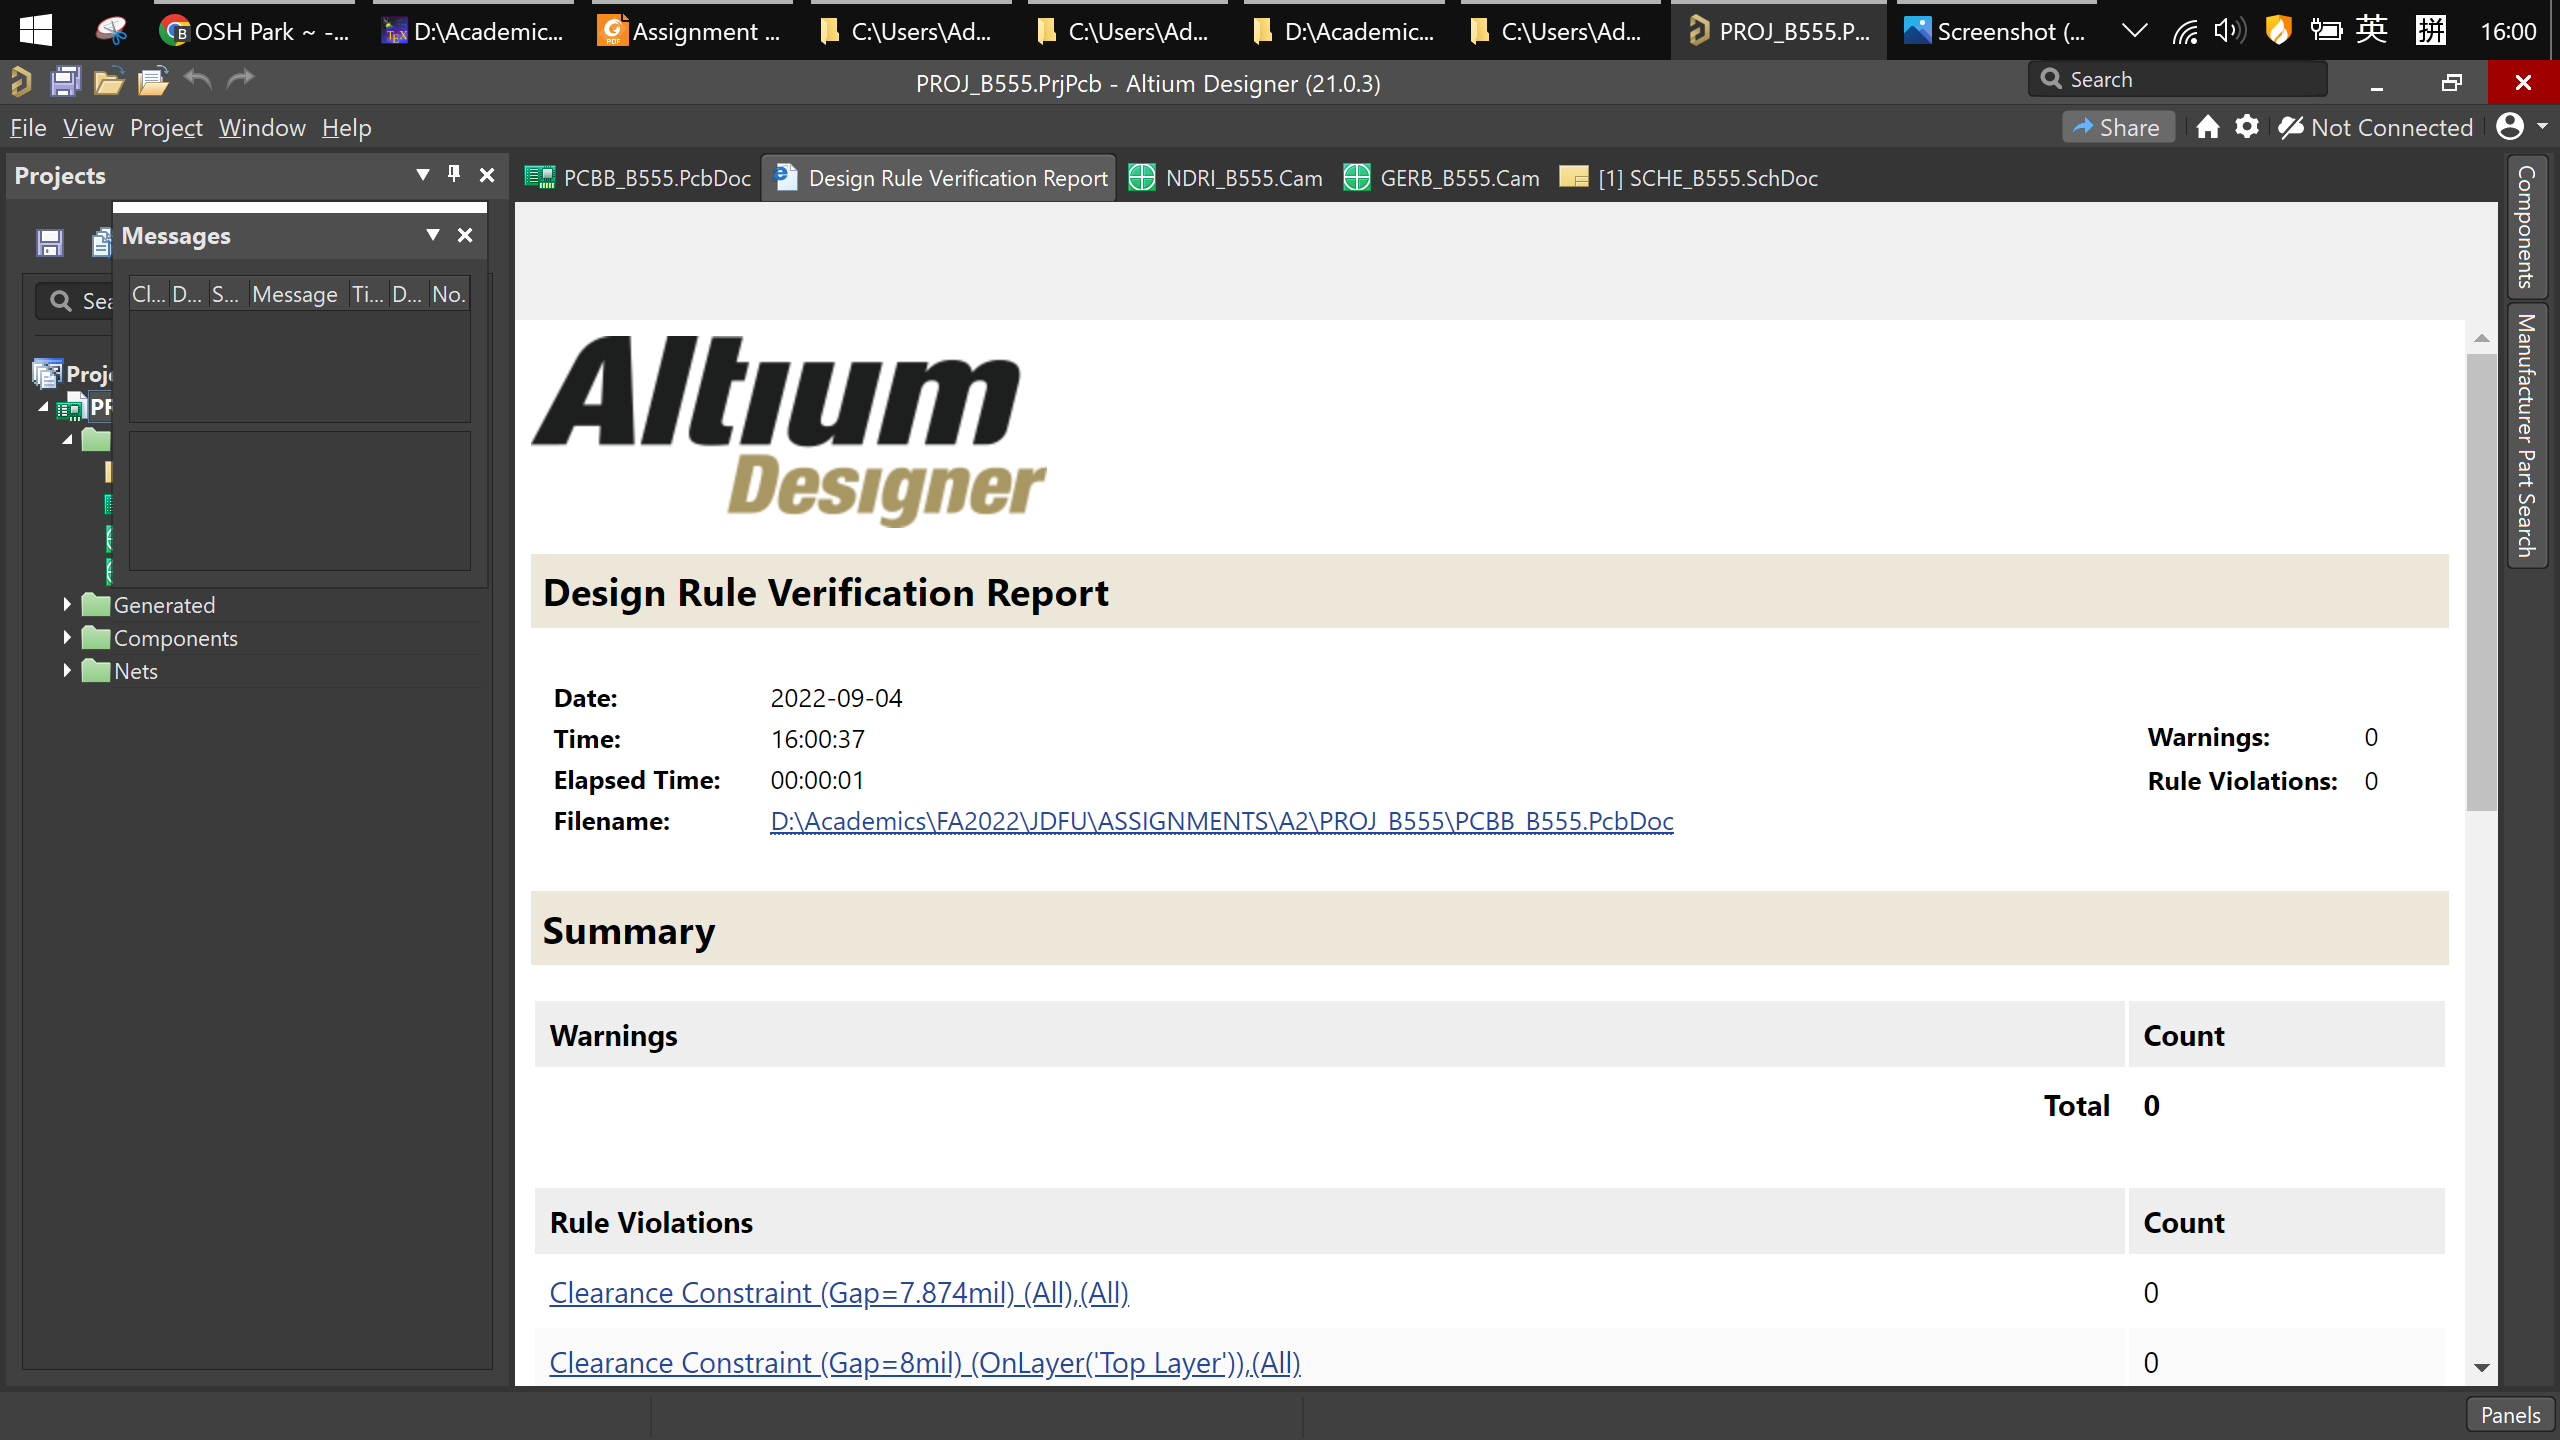
\includegraphics[width=\columnwidth]{DRVA_B555}
	\section{Screenshots of your BOM:}
	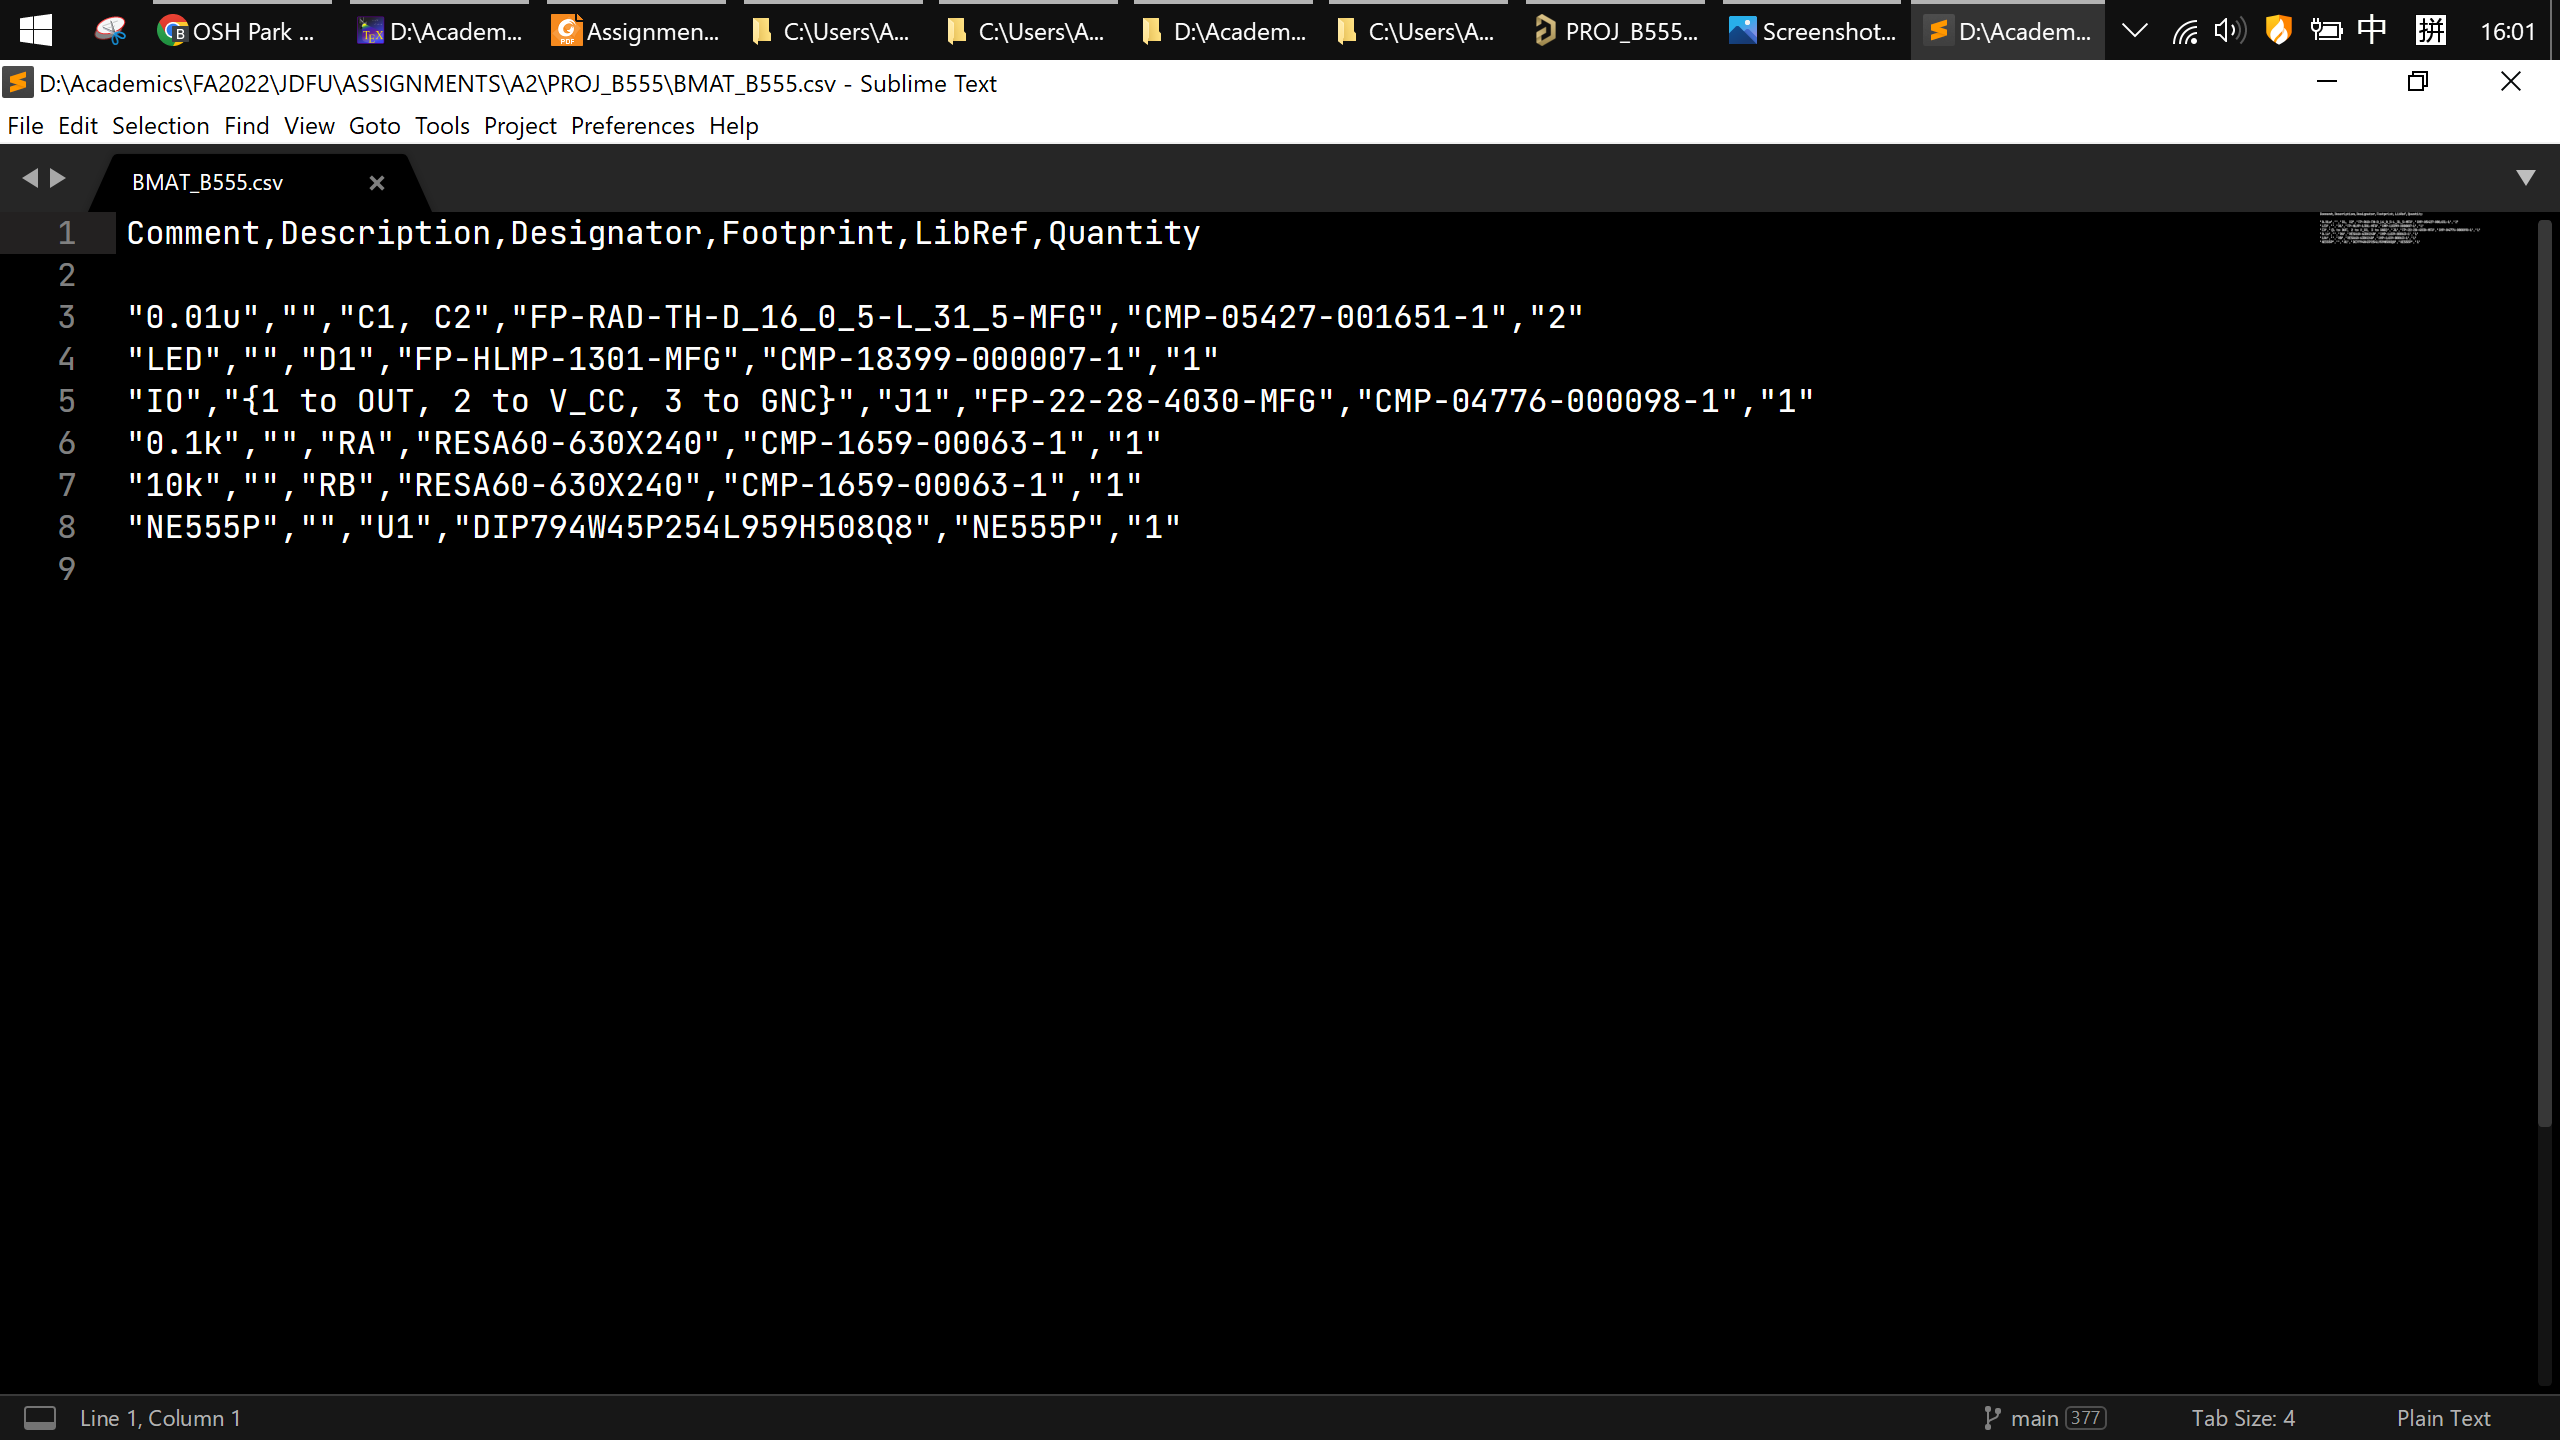
\includegraphics[width=\columnwidth]{BMAT_B555}
\end{document}